
%% bare_conf.tex
%% V1.4b
%% 2015/08/26
%% by Michael Shell
%% See:
%% http://www.michaelshell.org/
%% for current contact information.
%%
%% This is a skeleton file demonstrating the use of IEEEtran.cls
%% (requires IEEEtran.cls version 1.8b or later) with an IEEE
%% conference paper.
%%
%% Support sites:
%% http://www.michaelshell.org/tex/ieeetran/
%% http://www.ctan.org/pkg/ieeetran
%% and
%% http://www.ieee.org/

%%*************************************************************************
%% Legal Notice:
%% This code is offered as-is without any warranty either expressed or
%% implied; without even the implied warranty of MERCHANTABILITY or
%% FITNESS FOR A PARTICULAR PURPOSE!
%% User assumes all risk.
%% In no event shall the IEEE or any contributor to this code be liable for
%% any damages or losses, including, but not limited to, incidental,
%% consequential, or any other damages, resulting from the use or misuse
%% of any information contained here.
%%
%% All comments are the opinions of their respective authors and are not
%% necessarily endorsed by the IEEE.
%%
%% This work is distributed under the LaTeX Project Public License (LPPL)
%% ( http://www.latex-project.org/ ) version 1.3, and may be freely used,
%% distributed and modified. A copy of the LPPL, version 1.3, is included
%% in the base LaTeX documentation of all distributions of LaTeX released
%% 2003/12/01 or later.
%% Retain all contribution notices and credits.
%% ** Modified files should be clearly indicated as such, including  **
%% ** renaming them and changing author support contact information. **
%%*************************************************************************


% *** Authors should verify (and, if needed, correct) their LaTeX system  ***
% *** with the testflow diagnostic prior to trusting their LaTeX platform ***
% *** with production work. The IEEE's font choices and paper sizes can   ***
% *** trigger bugs that do not appear when using other class files.       ***                          ***
% The testflow support page is at:
% http://www.michaelshell.org/tex/testflow/



\documentclass[10pt,conference,compsocconf,letterpaper]{IEEEtran}
% Some Computer Society conferences also require the compsoc mode option,
% but others use the standard conference format.
%
% If IEEEtran.cls has not been installed into the LaTeX system files,
% manually specify the path to it like:
% \documentclass[conference]{../sty/IEEEtran}





% Some very useful LaTeX packages include:
% (uncomment the ones you want to load)
\usepackage{times}
\usepackage{cite}
\usepackage{url}
\usepackage{graphicx}
\usepackage{subfig}
\usepackage{multirow}
\usepackage{booktabs}
\usepackage{threeparttable}
\usepackage{algorithm}
\usepackage{algorithmic}
\renewcommand{\algorithmicrequire}{ \textbf{Input:}}
\renewcommand{\algorithmicensure}{ \textbf{Output:}}
\renewcommand{\arraystretch}{1.5}

% *** MISC UTILITY PACKAGES ***
%
%\usepackage{ifpdf}
% Heiko Oberdiek's ifpdf.sty is very useful if you need conditional
% compilation based on whether the output is pdf or dvi.
% usage:
% \ifpdf
%   % pdf code
% \else
%   % dvi code
% \fi
% The latest version of ifpdf.sty can be obtained from:
% http://www.ctan.org/pkg/ifpdf
% Also, note that IEEEtran.cls V1.7 and later provides a builtin
% \ifCLASSINFOpdf conditional that works the same way.
% When switching from latex to pdflatex and vice-versa, the compiler may
% have to be run twice to clear warning/error messages.






% *** CITATION PACKAGES ***
%
%\usepackage{cite}
% cite.sty was written by Donald Arseneau
% V1.6 and later of IEEEtran pre-defines the format of the cite.sty package
% \cite{} output to follow that of the IEEE. Loading the cite package will
% result in citation numbers being automatically sorted and properly
% "compressed/ranged". e.g., [1], [9], [2], [7], [5], [6] without using
% cite.sty will become [1], [2], [5]--[7], [9] using cite.sty. cite.sty's
% \cite will automatically add leading space, if needed. Use cite.sty's
% noadjust option (cite.sty V3.8 and later) if you want to turn this off
% such as if a citation ever needs to be enclosed in parenthesis.
% cite.sty is already installed on most LaTeX systems. Be sure and use
% version 5.0 (2009-03-20) and later if using hyperref.sty.
% The latest version can be obtained at:
% http://www.ctan.org/pkg/cite
% The documentation is contained in the cite.sty file itself.






% *** GRAPHICS RELATED PACKAGES ***
%
\ifCLASSINFOpdf
  % \usepackage[pdftex]{graphicx}
  % declare the path(s) where your graphic files are
  % \graphicspath{{../pdf/}{../jpeg/}}
  % and their extensions so you won't have to specify these with
  % every instance of \includegraphics
  % \DeclareGraphicsExtensions{.pdf,.jpeg,.png}
\else
  % or other class option (dvipsone, dvipdf, if not using dvips). graphicx
  % will default to the driver specified in the system graphics.cfg if no
  % driver is specified.
  % \usepackage[dvips]{graphicx}
  % declare the path(s) where your graphic files are
  % \graphicspath{{../eps/}}
  % and their extensions so you won't have to specify these with
  % every instance of \includegraphics
  % \DeclareGraphicsExtensions{.eps}
\fi
% graphicx was written by David Carlisle and Sebastian Rahtz. It is
% required if you want graphics, photos, etc. graphicx.sty is already
% installed on most LaTeX systems. The latest version and documentation
% can be obtained at:
% http://www.ctan.org/pkg/graphicx
% Another good source of documentation is "Using Imported Graphics in
% LaTeX2e" by Keith Reckdahl which can be found at:
% http://www.ctan.org/pkg/epslatex
%
% latex, and pdflatex in dvi mode, support graphics in encapsulated
% postscript (.eps) format. pdflatex in pdf mode supports graphics
% in .pdf, .jpeg, .png and .mps (metapost) formats. Users should ensure
% that all non-photo figures use a vector format (.eps, .pdf, .mps) and
% not a bitmapped formats (.jpeg, .png). The IEEE frowns on bitmapped formats
% which can result in "jaggedy"/blurry rendering of lines and letters as
% well as large increases in file sizes.
%
% You can find documentation about the pdfTeX application at:
% http://www.tug.org/applications/pdftex





% *** MATH PACKAGES ***
%
%\usepackage{amsmath}
% A popular package from the American Mathematical Society that provides
% many useful and powerful commands for dealing with mathematics.
%
% Note that the amsmath package sets \interdisplaylinepenalty to 10000
% thus preventing page breaks from occurring within multiline equations. Use:
%\interdisplaylinepenalty=2500
% after loading amsmath to restore such page breaks as IEEEtran.cls normally
% does. amsmath.sty is already installed on most LaTeX systems. The latest
% version and documentation can be obtained at:
% http://www.ctan.org/pkg/amsmath





% *** SPECIALIZED LIST PACKAGES ***
%
%\usepackage{algorithmic}
% algorithmic.sty was written by Peter Williams and Rogerio Brito.
% This package provides an algorithmic environment fo describing algorithms.
% You can use the algorithmic environment in-text or within a figure
% environment to provide for a floating algorithm. Do NOT use the algorithm
% floating environment provided by algorithm.sty (by the same authors) or
% algorithm2e.sty (by Christophe Fiorio) as the IEEE does not use dedicated
% algorithm float types and packages that provide these will not provide
% correct IEEE style captions. The latest version and documentation of
% algorithmic.sty can be obtained at:
% http://www.ctan.org/pkg/algorithms
% Also of interest may be the (relatively newer and more customizable)
% algorithmicx.sty package by Szasz Janos:
% http://www.ctan.org/pkg/algorithmicx




% *** ALIGNMENT PACKAGES ***
%
%\usepackage{array}
% Frank Mittelbach's and David Carlisle's array.sty patches and improves
% the standard LaTeX2e array and tabular environments to provide better
% appearance and additional user controls. As the default LaTeX2e table
% generation code is lacking to the point of almost being broken with
% respect to the quality of the end results, all users are strongly
% advised to use an enhanced (at the very least that provided by array.sty)
% set of table tools. array.sty is already installed on most systems. The
% latest version and documentation can be obtained at:
% http://www.ctan.org/pkg/array


% IEEEtran contains the IEEEeqnarray family of commands that can be used to
% generate multiline equations as well as matrices, tables, etc., of high
% quality.




% *** SUBFIGURE PACKAGES ***
%\ifCLASSOPTIONcompsoc
%  \usepackage[caption=false,font=normalsize,labelfont=sf,textfont=sf]{subfig}
%\else
%  \usepackage[caption=false,font=footnotesize]{subfig}
%\fi
% subfig.sty, written by Steven Douglas Cochran, is the modern replacement
% for subfigure.sty, the latter of which is no longer maintained and is
% incompatible with some LaTeX packages including fixltx2e. However,
% subfig.sty requires and automatically loads Axel Sommerfeldt's caption.sty
% which will override IEEEtran.cls' handling of captions and this will result
% in non-IEEE style figure/table captions. To prevent this problem, be sure
% and invoke subfig.sty's "caption=false" package option (available since
% subfig.sty version 1.3, 2005/06/28) as this is will preserve IEEEtran.cls
% handling of captions.
% Note that the Computer Society format requires a larger sans serif font
% than the serif footnote size font used in traditional IEEE formatting
% and thus the need to invoke different subfig.sty package options depending
% on whether compsoc mode has been enabled.
%
% The latest version and documentation of subfig.sty can be obtained at:
% http://www.ctan.org/pkg/subfig




% *** FLOAT PACKAGES ***
%
%\usepackage{fixltx2e}
% fixltx2e, the successor to the earlier fix2col.sty, was written by
% Frank Mittelbach and David Carlisle. This package corrects a few problems
% in the LaTeX2e kernel, the most notable of which is that in current
% LaTeX2e releases, the ordering of single and double column floats is not
% guaranteed to be preserved. Thus, an unpatched LaTeX2e can allow a
% single column figure to be placed prior to an earlier double column
% figure.
% Be aware that LaTeX2e kernels dated 2015 and later have fixltx2e.sty's
% corrections already built into the system in which case a warning will
% be issued if an attempt is made to load fixltx2e.sty as it is no longer
% needed.
% The latest version and documentation can be found at:
% http://www.ctan.org/pkg/fixltx2e


%\usepackage{stfloats}
% stfloats.sty was written by Sigitas Tolusis. This package gives LaTeX2e
% the ability to do double column floats at the bottom of the page as well
% as the top. (e.g., "\begin{figure*}[!b]" is not normally possible in
% LaTeX2e). It also provides a command:
%\fnbelowfloat
% to enable the placement of footnotes below bottom floats (the standard
% LaTeX2e kernel puts them above bottom floats). This is an invasive package
% which rewrites many portions of the LaTeX2e float routines. It may not work
% with other packages that modify the LaTeX2e float routines. The latest
% version and documentation can be obtained at:
% http://www.ctan.org/pkg/stfloats
% Do not use the stfloats baselinefloat ability as the IEEE does not allow
% \baselineskip to stretch. Authors submitting work to the IEEE should note
% that the IEEE rarely uses double column equations and that authors should try
% to avoid such use. Do not be tempted to use the cuted.sty or midfloat.sty
% packages (also by Sigitas Tolusis) as the IEEE does not format its papers in
% such ways.
% Do not attempt to use stfloats with fixltx2e as they are incompatible.
% Instead, use Morten Hogholm'a dblfloatfix which combines the features
% of both fixltx2e and stfloats:
%
% \usepackage{dblfloatfix}
% The latest version can be found at:
% http://www.ctan.org/pkg/dblfloatfix




% *** PDF, URL AND HYPERLINK PACKAGES ***
%
%\usepackage{url}
% url.sty was written by Donald Arseneau. It provides better support for
% handling and breaking URLs. url.sty is already installed on most LaTeX
% systems. The latest version and documentation can be obtained at:
% http://www.ctan.org/pkg/url
% Basically, \url{my_url_here}.




% *** Do not adjust lengths that control margins, column widths, etc. ***
% *** Do not use packages that alter fonts (such as pslatex).         ***
% There should be no need to do such things with IEEEtran.cls V1.6 and later.
% (Unless specifically asked to do so by the journal or conference you plan
% to submit to, of course. )


% correct bad hyphenation here
\hyphenation{op-tical net-works semi-conduc-tor}


\begin{document}
%
% paper title
% Titles are generally capitalized except for words such as a, an, and, as,
% at, but, by, for, in, nor, of, on, or, the, to and up, which are usually
% not capitalized unless they are the first or last word of the title.
% Linebreaks \\ can be used within to get better formatting as desired.
% Do not put math or special symbols in the title.
\title{Lever: Towards Low-Latency Batched Stream Processing by Pre-Scheduling}


% author names and affiliations
% use a multiple column layout for up to three different
% affiliations
%\author{\IEEEauthorblockN{Fei Chen\IEEEauthorrefmark{1}, Song Wu\IEEEauthorrefmark{1}, Hai Jin\IEEEauthorrefmark{1}, Yongluan Zhou\IEEEauthorrefmark{2}, Lin Gu\IEEEauthorrefmark{1}, Yin Yao\IEEEauthorrefmark{1}, Zhiyi Liu\IEEEauthorrefmark{1}}

%\IEEEauthorblockA{\IEEEauthorrefmark{1} SCTS/CGCL, Huazhong University of Science and Technology, China}

%\IEEEauthorblockA{\IEEEauthorrefmark{2} University of Southern Denmark, Denmark}
%}
\author{Fei Chen$^1$, Song Wu$^1$, Hai Jin$^1$, Yongluan Zhou$^2$, Lin Gu$^1$, Yin Yao$^1$ and Zhiyi Liu$^1$ \\
\small{\em $^1$SCTS/CGCL, Huazhong University of Science and Technology, China \quad
           $^2$University of Southern Denmark, Denmark} \\ [2mm]
\small Submission Type: Research
}
\date{}

% conference papers do not typically use \thanks and this command
% is locked out in conference mode. If really needed, such as for
% the acknowledgment of grants, issue a \IEEEoverridecommandlockouts
% after \documentclass

% for over three affiliations, or if they all won't fit within the width
% of the page, use this alternative format:
%
%\author{\IEEEauthorblockN{Michael Shell\IEEEauthorrefmark{1},
%Homer Simpson\IEEEauthorrefmark{2},
%James Kirk\IEEEauthorrefmark{3},
%Montgomery Scott\IEEEauthorrefmark{3} and
%Eldon Tyrell\IEEEauthorrefmark{4}}
%\IEEEauthorblockA{\IEEEauthorrefmark{1}School of Electrical and Computer Engineering\\
%Georgia Institute of Technology,
%Atlanta, Georgia 30332--0250\\ Email: see http://www.michaelshell.org/contact.html}
%\IEEEauthorblockA{\IEEEauthorrefmark{2}Twentieth Century Fox, Springfield, USA\\
%Email: homer@thesimpsons.com}
%\IEEEauthorblockA{\IEEEauthorrefmark{3}Starfleet Academy, San Francisco, California 96678-2391\\
%Telephone: (800) 555--1212, Fax: (888) 555--1212}
%\IEEEauthorblockA{\IEEEauthorrefmark{4}Tyrell Inc., 123 Replicant Street, Los Angeles, California 90210--4321}}




% use for special paper notices
%\IEEEspecialpapernotice{(Invited Paper)}




% make the title area
\maketitle

% As a general rule, do not put math, special symbols or citations
% in the abstract
\begin{abstract}

  Many stream processing frameworks have been developed to meet the requirements of real-time processing. Among them, batched stream processing frameworks are widely advocated with the consideration of their fault-tolerance and high throughput. In batched stream processing frameworks , straggler, happened due to the uneven task execution time, has been regarded as a major hurdle of latency-sensitive applications. Existing straggler mitigation techniques, operating in either reactive or proactive manner, are all post-scheduling methods, and therefore may inevitably result in high resource overhead or long job completion time. We notice that batched stream processing jobs are usually recurring with predictable characteristics. By exploring such feature, we present a pre-scheduling straggler mitigation framework called Lever. Lever first identifies potential stragglers and evaluates nodes' capability by analyzing execution information of historical jobs. Then, Lever carefully pre-schedules job input data to each node before task scheduling so as to mitigate the potential stragglers. We implement Lever and contribute it as an extension of Apache Spark Streaming. Our experimental results show that Lever can reduce job completion time by 30.72\% to 42.19\% over Spark Streaming, a widely adopted batched stream processing system and outperforms traditional techniques significantly.

\end{abstract}

\begin{IEEEkeywords}
stream processing; recurring jobs; straggler; scheduling; data assignment

\end{IEEEkeywords}
% no keywords

% For peer review papers, you can put extra information on the cover
% page as needed:
% \ifCLASSOPTIONpeerreview
% \begin{center} \bfseries EDICS Category: 3-BBND \end{center}
% \fi
%
% For peerreview papers, this IEEEtran command inserts a page break and
% creates the second title. It will be ignored for other modes.
\IEEEpeerreviewmaketitle

\section{Introduction}
% no \IEEEPARstart
% You must have at least 2 lines in the paragraph with the drop letter
% (should never be an issue)

  With the vast involvement of streaming big data in many applications (e.g., stock market data, sensor data, social network data, etc.), quickly mining and analyzing such data is becoming more and more important. There is a recent trend in adapting batch-based data processing systems, such as MapReduce \cite{Dean2004} and Spark \cite{Zaharia2010C}, to handle streaming data by putting the input streams into micro-batches and treating the workloads as a continuous series of small jobs. Examples of such systems include HOP \cite{Condie2010}, Comet \cite{He2010}, HStreaming \cite{HStreaming} and Spark Streaming \cite{Zaharia2013}. Figure 1 illustrates a simplified model of the data handling pipeline in such systems. In this model, the \emph{batching module} receives and divides the data streams into batches. Then, these batches are put into the \emph{batch queue}. The \emph{processing module} schedules tasks for processing according to the (BSP) model.
  \begin{figure}[htbp]
    \centering
    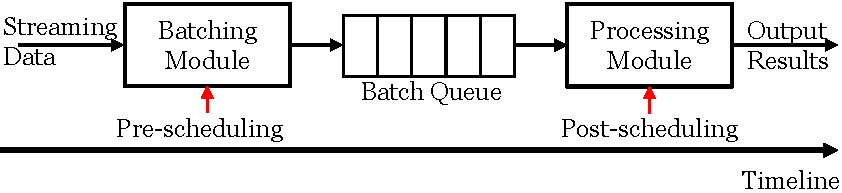
\includegraphics[width=0.40\textwidth]{FigureModel}
    \caption{Model of a batched stream processing system}\label{Fig. 1:}
  \end{figure}

  Batched stream processing systems become popular because not only they provide a unified programming model to process batch data and streaming data, but also they can leverage the fault tolerance and high throughput properties of the batch processing frameworks \cite{spark-summit}. However, in comparing to record-at-a-time stream processing systems, such as Storm \cite{storm-web}, and Naiad \cite{Murray2013}, batched steam processing systems often suffer from high processing latency. Therefore, the fundamental challenge of building a batched stream processing system is how to minimize the processing latency of each micro-batch. This problem has recently attracted the community's interest, and some efforts, such as Drizzle \cite{drizzle}, have been focused on minimizing the coordination overhead of processing the micro-batches, including the cost incurred by task scheduling and barriers between different processing stages.

  In this paper, we focus on another issue, namely the straggler problem, where a subset of workers straggling behind and significantly affecting the job completion time. The straggler problem is a well-known critical problem in parallel processing systems. As reported in \cite{Ananthanarayanan2013} and \cite{Yadwadkar2014}, in the production clusters at Facebook and Microsoft Bing, straggler tasks are on average 8 times slower than the median task in the same job.

  In comparing to processing of large batches, the straggler problems in micro-batch processing are more severe and harder to tackle. First of all, unlike processing large batches, where there are multiple waves of tasks to be scheduled, the number of tasks in micro-batch processing is much more limited, therefore, once a straggler occurs, we have little opportunity to amortize the influence of straggler. Second, small batched streaming jobs are strictly latency-sensitive(processing time $<$ batch interval). Batched stream processing system handle many continuously recurring micro-batches, if the execution times of the straggling tasks exceed the batch interval, it would not only affect the latency of the current micro-batch, but also the subsequent ones, which would suffer from unacceptable queueing latency. Furthermore, the actions of handling stragglers have to be carried out very quickly so that the total task (re-)scheduling and processing time should not exceed the batch interval. This is especially challenging if we use small, say sub-second, batch intervals. For example, the wait-speculate-re-execute paradigm adopted in many existing solutions \cite{Dean2004} \cite{Zaharia2008} \cite{Kwon2012} would be undesirable, because the processing time of the micro-batches can be too short to afford the waiting time to detect the stragglers, not to mention the additional latency incurred by relocating the data and re-executing the straggling tasks.

  We argue that the fundamental problem of using the existing straggler mitigation solutions for micro-batch processing is that they detect (or predict) stragglers and reschedule them too late in the data handling pipeline, i.e. after the batching module has already dispatched the data into the batch queue and the processing module has started processing the data (recall Figure 1). The re-scheduling actions are carried out during the task execution period, hence it would inevitably increase the processing time of the micro-batches. Furthermore, as the data have already been dispatched, re-scheduling would inherently incur expensive data relocation. Such overhead would become significant in micro-batch processing due to the short processing time of each micro-batch. We refer to this type of methods as \emph{post-scheduling} techniques.

  To address the problem, we propose a new \emph{pre-scheduling} framework, called \emph{Lever}, which predicts stragglers and makes timely scheduling decisions to minimize the processing latency. Lever utilizes the statistics of the processing of the previous batches to predict the potential stragglers in the current batch and makes proactive re-scheduling decisions to prevent stragglers. More specifically, Lever makes the re-scheduling decisions before the batching module dispatches the data. Therefore, the re-scheduling actions would not incur any data relocation, and, as the scheduling is done while the data are being batched, it would not increase the processing time of the micro-batch.

  We implemented Lever in Spark Streaming, which is contributed to the open source community as an extension of Apache Spark Streaming. To the best of our knowledge, this is the first work specifically addressing the straggler problem in continuous micro-batch processing. In summary, this paper makes the following technical contributions:

\begin{itemize}
  \item We discuss the behaviors of existing straggler mitigation methods and identify the problems of existing straggler mitigation methods for batched stream processing systems.

  \item To better mitigate stragglers when processing micro-batches, we present Lever, a pre-scheduling framework for handling straggler problems in batched stream processing systems. Lever predicts and pre-schedules straggling tasks when dispatching the data to avoid the latency incurred by the post-scheduling methods. Furthermore, by mitigating the stragglers, Lever can significantly reduce the processing latency of micro-batches.

  \item We propose various techniques to realize the new pre-scheduling framework. We propose a method to predict the potential stragglers before the execution of the tasks by using the historical statistics, which takes into account the variations of data streaming rates. In addition, we adopt the Iterative Learning Control model to estimate the capability of the computing nodes. Finally, we propose two techniques to pre-schedule the straggling tasks, which are suitable for a small and a large number of stragglers respectively. A method is proposed to automatically choose one out of these two techniques according the actual situation.

  \item We implemented Lever on Spark Streaming, and contributed it as an extension of Spark Streaming to the open source community. Extensive experiments using both real and synthetic data show that Lever can mitigate stragglers efficiently and improve the performance of stream applications significantly.
\end{itemize}

  The rest of this paper is organized as follows. In Section II, we introduce the background and analyze the straggler problems in batched stream processing system. Section III describes the pre-scheduling strategy and the design of Lever. Section IV presents the implementation of Lever. We evaluate the performance of our system in Section V. Section VI briefly surveys the related works. Finally, Section VII concludes this paper.

\section{Background and Motivation}

  In this section, we first introduce the background of batched stream processing and stragglers. Then we deep into the problems existing in traditional straggler mitigation strategies when processing short stream jobs. We also briefly analyze the characteristics of recurring batched stream jobs. Finally, we outline the challenges in pre-scheduling straggler mitigation.

\subsection{Background}

  Batched stream processing system treats a streaming computation as a series of deterministic batch computations on small time intervals \cite{Zaharia2013}. As shown in Figure 2, batched stream processing system (1) receives input data and divides continuous data stream into a series of small batches according to batch interval (a time granularity which is set according to application's response time), (2) when each batch interval arrives, batch jobs are generated for each batch, (3) these jobs would be repeatedly submitted to batch processing engine such as MapReduce or Spark and are re-run periodically to execute with distributed fault tolerance, data locality scheduling and load balancing provided by batch framework automatically. Latency sensitive, micro jobs/tiny tasks and recurring jobs are three dominant characteristics of these systems.
  \begin{figure}[htbp]
    \centering
    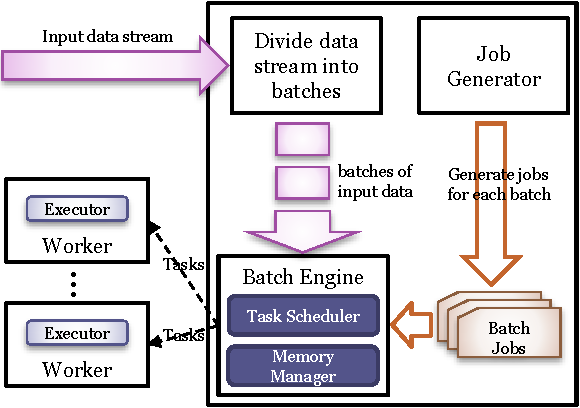
\includegraphics[width=0.34\textwidth]{FigureBatchStream}
    \caption{Principles of batched stream processing system}\label{Fig. 2:}
  \end{figure}

  Stragglers have been a primary performance issue for batched stream processing system. Because the whole job must wait for the slowest task. These stragglers cause unproductive wait time for all the others, delaying job completion. Stragglers especially impact short batched stream jobs. On the one hand, short batched stream jobs are more latency-sensitive and require short response time. On the other hand, short batched stream jobs consist of just a few tasks. Such jobs typically get to run all their tasks at less waves. So, if one task straggles, the whole job is significantly delayed. Beyond these, if a job is so severely affected by stragglers that its completion time exceeds one batch interval, it will delay the next job's submission and execution. Stragglers can occur for many reasons, including hardware heterogeneity \cite{Reiss2012}, data skew \cite{Kwon2012}, hardware failures \cite{Ananthanarayanan2010}, energy efficiency \cite{Cheng2015}, resource contention and various OS effects.

\subsection{Problem Analysis}

  Existing methods to straggler mitigation are post-scheduling methods. They fall short in multiple ways. In the following, we analyze four representative approaches. They are Speculative execution, SkewTune, Dolly and Wrangler on behalf of reactive approach with replication, reactive approach without replication, proactive approach with replication and proactive approach without replication respectively.
  \begin{figure*}[htbp]
    \centering
    \subfloat[Speculative Execution]{%
      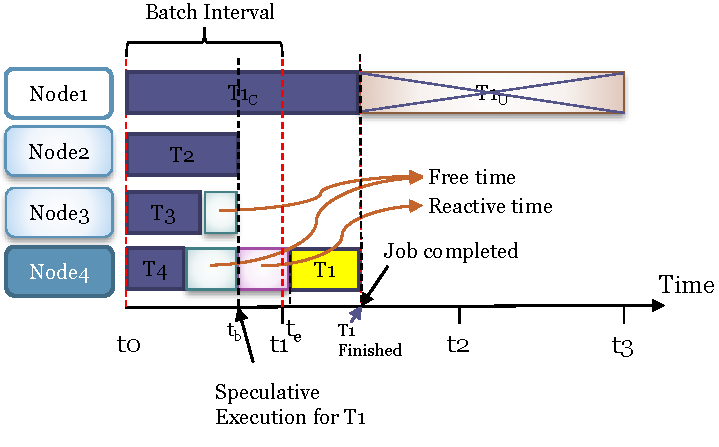
\includegraphics[width=0.42\textwidth]{Figure5a}
    }
    \subfloat[SkewTune]{%
      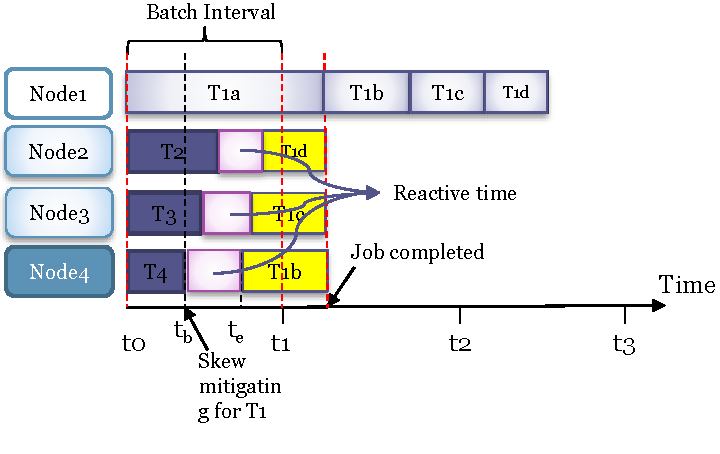
\includegraphics[width=0.42\textwidth]{Figure5b}
    }\hfill
    \subfloat[Dolly]{%
      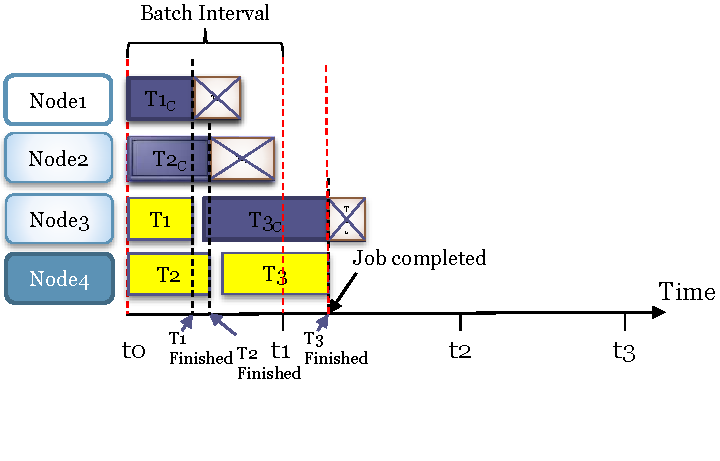
\includegraphics[width=0.42\textwidth]{Figure5c}
    }
    \subfloat[Wrangler]{%
      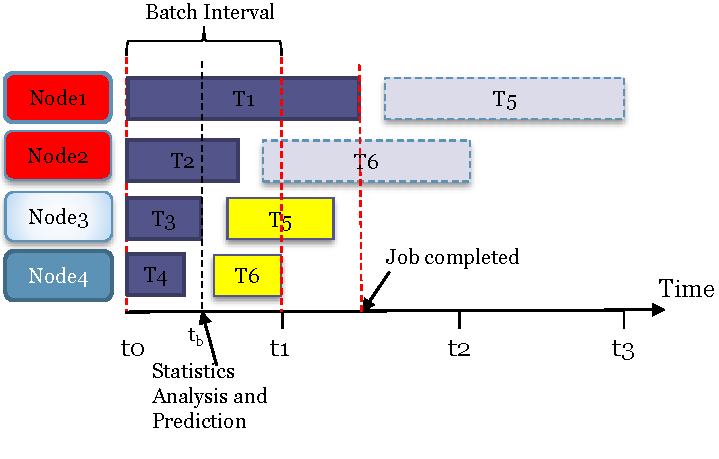
\includegraphics[width=0.42\textwidth]{Figure5d}
    }\hfill
    \caption{Straggler mitigation under different strategies}
    \label{Fig. 3:}
  \end{figure*}

  Reactive approaches rely on a wait-speculate-re-execute mechanism. Speculative execution \cite{Dean2004} is a widely used reactive approach with replication for straggler mitigation. Speculative execution marks slow running tasks as stragglers and reacts by re-launching multiple copies of them. As soon as one of these copies finishes execution, the rest are killed. Taking Fig. 3(a) as an example, at $t_b$, T1 is marked as stragglers. Then speculative execution launches a copy of T1 on node4. It migrates data block of Task T1 to node4 and starts executing at $t_e$. As we can see, this approach incurs long reactive time and free time for other nodes. It becomes inefficient for short batched stream jobs in two aspects. On one hand, a task must run for a significant amount of time before it can be identified as a straggler. By this time, other tasks of that job have made considerable progress already. On the other hand, the reaction procedure is time-consuming in the context of short stream job with only several seconds of response time, which is at the same magnitude of the time for speculation and migration.

  SkewTune \cite{Kwon2012} is  a reactive approach  without replication. Once one node has an available slot, SkewTune begins to detect data skew and identify stragglers according to each task's remaining time. As shown in Fig. 3(b), when task $T_4$ is completed at $t_b$, SkewTune's detection is triggered and $T_1$ is identified as straggler. Then, $T_1$ is selected for skew mitigation due to its long remaining progress. After that, SkewTune scans $T_1$'s remaining input data and repartitions its remaining workload into $T_{1b}$, $T_{1c}$ and $T_{1d}$, which  are  migrated to nodes $node_4$, $node_3$ and $node_2$, respectively. From $t_b$ to $t_e$, this procedure incurs approximately 2 seconds overhead for a task with 2MB's input data. This overhead grows linearly with the size of the task's input data, and is intolerant for short stream jobs which must be completed in several seconds or sub-seconds. Furthermore, before SkewTune begins, task $T_1$ has already slowed down. Therefore, basically SkewTune is also in wait-and-speculate paradigm.

  Dolly \cite{Ananthanarayanan2013} is a proactive strategy by full cloning of small jobs. Dolly launches multiple clones of every task of a job and only use the result of the clone that finishes first. As shown in Fig. 3(c), Dolly launches two clones of Task $T_1$ and $T_2$ in $node_1, node_3$ and $node_2, node_4$ respectively. After $T_1$ and $T_2$ complete, Dolly schedules $T_3$ and also launches two clones in $node_3$ and $node_4$. Although multiple clones for each task are spawned, only one of them is effective, incurring significant waste of resources.

  Unlike Dolly, Wrangler \cite{Yadwadkar2014} is a proactive strategy without replication. It predicts stragglers using an interpretable linear modeling technique based on cluster resource usage counters and uses these predictions to inform scheduling decisions. For example, in Fig. 3(d), Wrangler analyzes statistics and make predictions about stragglers at $t_b$. Node1 and node2 are identified as stragglers. Then Wrangler schedules and migrates T5 in node1, T6 in node2 onto node3 and node4 respectively. Although this approach can avoid successor possible stragglers, it remains taking hysteretic actions for short batched stream jobs. Because short batched stream jobs always consist of a few tasks and get to run at once. Furthermore, Wrangler can't act until some nodes show some indications of stragglers(eg. high cpu utilization, heavy memory access, network congestion). It also need to migrate data block at runtime regardless of data locality.

  In summary, existing post-scheduling approaches fall short when processing short stream jobs. Reactive approaches act after stragglers have occurred. At that time, tasks have already slowed down. Replication-based proactive approaches incur extra resource and increase 2x load. Proactive approaches without replication also need to migrate data block at runtime. Consequently, it is desirable to design a straggler mitigation strategy that can react as early as possible, without incurring too much extra resource overhead.

\subsection{Recurring Batched Stream Jobs}

  Batched stream jobs are periodic in nature, hence are typically recurring with stable code and data properties. Many characteristics, such as application logic, stragglers, resource utilization, scheduling and other operations, are statistically similar to the previous execution when running on newer data of the same stream \cite{Agarwal} \cite{Grandl2016} \cite{Jyothi2016}. The history of prior runs for recurring jobs can be used to estimate tasks' durations and predict stragglers.

  Considering the following two points that 1) Straggler characteristics can often be accurately predicted in recurring jobs and 2) Job input data can be assigned in designated locations before scheduling to avoid straggler in advance, we can try to mitigate stragglers via pre-scheduling by exploring the statistical similarity in short batched stream jobs.

\subsection{Challenges}

  We are faced with three challenges:

  Challenge 1 How to identify potential stragglers?

  Pre-scheduling need to know which nodes will be stragglers in next batch. Unlike traditional post-scheduling ways which identify stragglers based on runtime-aware decisions, pre-scheduling takes actions in batching model without task scheduling information. All that pre-scheduling can use is the historical information of recurring jobs. But only analyzing historical information is not enough due to the variability of stream load. Accurately identifying potential stragglers is a prerequisite step for eliminating stragglers.

  Challenge 2 How to determine node's capability?

  Traditional post-scheduling methods have resource utilization view at runtime and can schedule straggler tasks to that node which has free slots. However, in pre-scheduling solutions, it is impossible because we make pre-scheduling decisions before task scheduling. We should define a metric to determine how much data we should pre-schedule to target node. This metric represents to which degree this node will has free slots in future scheduling. So we introduce the notion of node's capability.

  Challenges 3 How to select suitable helpers for data assignment?

  To pre-schedule input data as evenly as possible to eliminate stragglers, pre-scheduling need to choose some helpers which are eligible to provide assistance. These helpers should be underloaded and have spare capability in next batch to deal with extra work assigned to them. As explained in Challenge 2, pre-scheduling don't have the perspective of runtime resource utilization. It brings great challenges when we make decisions about which nodes can afford extra load. How to choose suitable helpers with being unaware of task scheduling is a challenging problem.

  \begin{figure}[htbp]
    \centering
    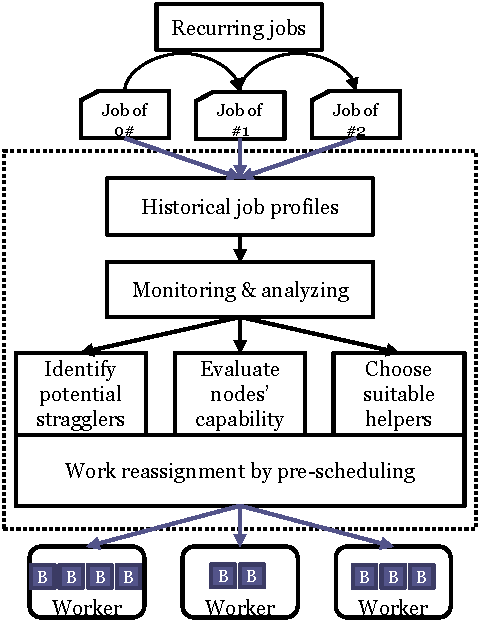
\includegraphics[width=0.35\textwidth]{FigureArchitecture}
    \caption{Architecture of Lever}
    \label{Fig. 4:}
  \end{figure}
  To overcome these challenges, we design and implement a prototype of Lever.

\section{System Design}

  In this section, we describe the design of Lever. Lever is designed to be API-compatible with Spark Streaming, providing the mitigation transparency and developer transparency. Considering the main objective is to lower latency, Lever is lightweight. We begin with an overview of the system architecture, followed by introducing the system details.

\subsection{System Overview}

  Figure 4 overviews the architecture of Lever. Lever periodically collects and analyzes the historical jobs' profiles of recurring batched streaming jobs. Based on these analysis, Lever pre-schedules job input data through three main steps, i.e. identify potential stragglers, evaluate nodes' capability and choose suitable helpers. Firstly, comparing each node's task finish time in previous batch, Lever can initially determine initial state of each node. Lever also estimates the changes of input data rate. Combined with these two aspects, Lever conduct state transition to decide which nodes will behaviors as stragglers in next batch(for Challenge 1). Secondly, based on the fact that batched stream processing jobs are repetitive and periodic, Lever introduces Iterative Learning Control (ILC \cite{Arimoto}), which is designed to do tracking control for systems that work in a repetitive mode to learn to estimate node's capability (for Challenge 2). Finally, considering that Lever don't have resource utilization view when pre-scheduling, Lever can choose all nodes or two least load nodes as helpers. Lever can adaptively switch between these two strategies to pursue high performance(for Challenge 3).

  We show the actions timing diagram of Lever in Figure 5, where we differentiate pre-scheduling and post-scheduling according to their scheduling timing. It can be seen that post-scheduling (e.g., Dolly, Wrangler, Speculation\&SkewTune) acts during processing but Lever, as a pre-scheduling approach, acts before task scheduling. As shown in Figure 5, Lever collects the needed information of the previous job's execution during batch interval between $t_1$ and $t_2$.
  Then, during $t_2$ and $t_3$, Lever pre-schedules input data based on prior pre-scheduling plan. When come to batch $t_3$ to $t_4$, Lever schedules tasks according to data locality as usual. We detail each step of Lever in the following.
  \begin{figure*}[htbp]
    \centering
    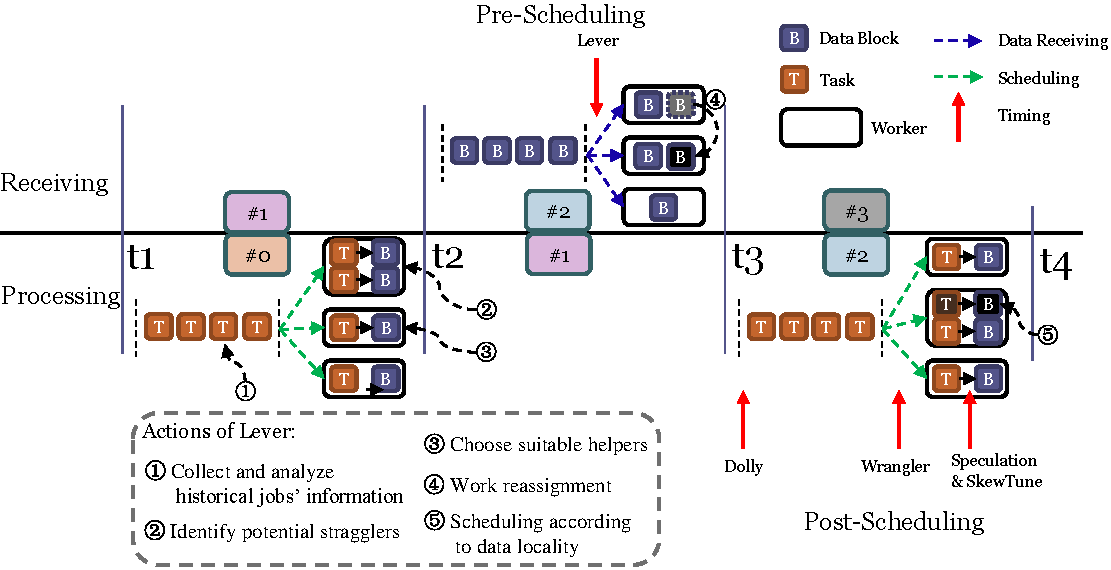
\includegraphics[width=0.8\textwidth]{FigureAction}
    \caption{Actions of Lever}
    \label{Fig. 5:}
  \end{figure*}

\subsection{Identify Potential Stragglers}

  Lever predicts stragglers in the next batch according to recurring jobs' historical execution information combined with the load fluctuation of each node. The first step is to determine the initial stragglers. When last batch's jobs are completed, Lever collects and analyze the statistics of tasks' execution information in each node. The node i's finish time ($NFT_i$) is defined as the time from job's submission to the last task finish in this node. Then, Lever sorts node's list according to $NFT_i$ in the descending order. It classify nodes into three categories according to two locations 0.25, 0.75(we refer to the quantile of speculation \cite{Dean2004}) of node's list size. Nodes before 0.25$\times$size are grouped into \emph{straggler group}. Nodes after 0.75$\times$size are grouped into \emph{faster group}. The remaining are categorized as \emph{median group}.

  This classification can only represent the stragglers in the last batch. Because stream load varies over time, i.e., load fluctuation, the state of each node may be different between two consecutive jobs. Therefore, we shall carefully derive the possible state transitions to accurately identify the stragglers as follows. First, Lever calculates the median finish time of \emph{straggler group}, \emph{median group} and \emph{faster group} respectively, represented as \emph{FTOS}, \emph{FTOM}, \emph{FTOF}. Second, Lever introduces degradation ratio \emph{FTM} and \emph{MTS}. \emph{FTM} is defined as \emph{FTOM}/\emph{FTOF}. It means that if one node's $NFT_i$ in \emph{faster group} has increased by FTM, it will be moved from \emph{faster group} to \emph{median group} and vice versa. Similarly, \emph{MTS} is defined as \emph{FTOS}/\emph{FTOM}. It means that if one node's $NFT_i$ in \emph{median group} has increased by MTS, it will be moved from \emph{median group} to \emph{straggler group} and vice versa. We have shown straggler's state transition in Fig. 6.
  \begin{figure}[htbp]
    \centering
    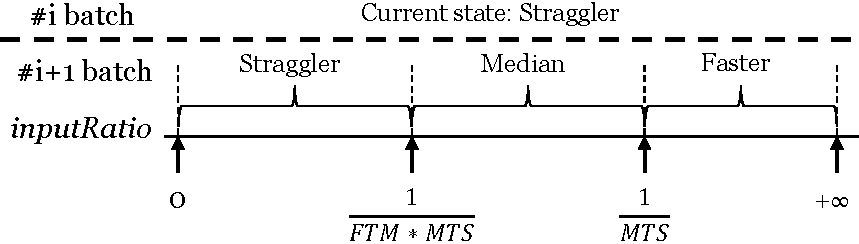
\includegraphics[width=0.42\textwidth]{FigureI2}
    \caption{An example for straggler's state transition}
    \label{Fig. 6:}
  \end{figure}

  Based on the transition graph in Fig. 6, in the third step, Lever takes the load fluctuation observed on each node to conduct state transition for straggler identification. Due to the load fluctuation, last batch's stragglers may receive less data and hence become faster in current batch. Similarly, the faster nodes may also possibly becom stragglers in current batch. Lever introduces \emph{inputRatio} as the ratio between the new input data rate of current batch and the old one of the last batch to evaluate the changes of stream load. According to the transition graph, we define the transition rules in Table \uppercase\expandafter{\romannumeral1}, by applying which Lever finally identifies the state of each node for current batch.
  \begin{table}[htbp]
    \footnotesize
    \centering
    \caption{Transition rules for identifying stragglers}
    \begin{threeparttable}
    \centering
      \begin{tabular}{|p{1.5cm}|p{4.3cm}|p{1.4cm}|}
        \hline
        Initial State & Transition Conditions(inputRatio) & Final State \\
        \hline
        \multirow{3}{2cm}{Straggler} &
        (1/MTS,$+\infty$) & Straggler \\
        \cline{2-3}
        & [1/(FTM*MTS),1/MTS] & Median \\
        \cline{2-3}
        & (0,1/(FTM*MTS)) & Faster \\
        \hline
        \multirow{3}{2cm}{Median} &
        (MTS,$+\infty$) & Straggler \\
        \cline{2-3}
        & [1/FTM,MTS] & Median \\
        \cline{2-3}
        & (0,1/FTM) & Faster \\
        \hline
        \multirow{3}{2cm}{Faster} &
        (FTM*MTS,$+\infty$) & Straggler \\
        \cline{2-3}
        & [FTM,FTM*MTS] & Median \\
        \cline{2-3}
        & (0,FTM) & Faster \\
        \hline
      \end{tabular}
    \end{threeparttable}
    \label{Table1}
  \end{table}

\subsection{Computational Capability Determination}

  After determine the state of each node according to the input data characteristics, we next evaluate each node's computational capability so as to conduct pre-scheduling, as detailed in this section.

\subsubsection{Computational Capability}

  The computational capability is defined as the metric which one node can process how much data in one batch. As shown in Section \uppercase\expandafter{\romannumeral2}-C, recurring batched stream jobs have stable data properties. By analyzing the previous execution, We can assess these metrics exactly in the subsequent execution.

  Considering the periodicity of recurring batched stream jobs, we evaluate computational capability based on a well-known optimization technique, Iterative Learning Control (ILC \cite{Arimoto}), which is designed to do tracking control for systems that work in a repetitive mode. Repetition allows the system to improve tracking accuracy from repetition to repetition. This learning process uses information from previous repetitions to improve the estimation ultimately enabling a more and more accurate result can be found iteratively. This scenario is similar to batched stream processing jobs.
  \begin{figure}[htbp]
    \centering
    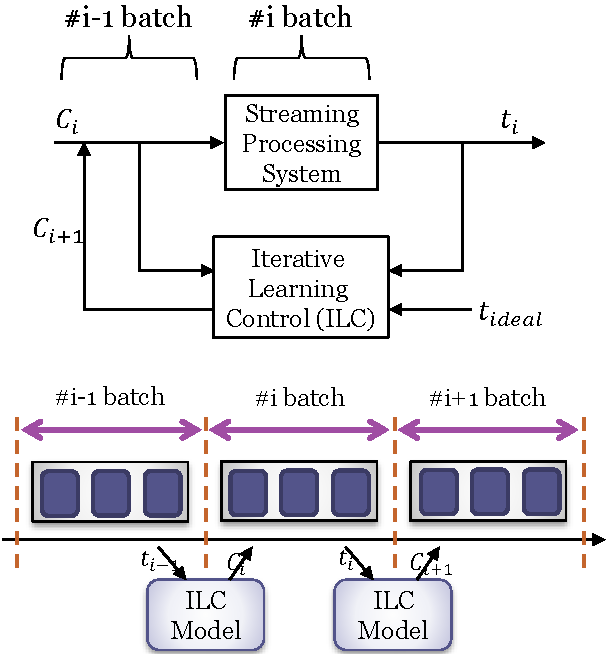
\includegraphics[width=0.36\textwidth]{FigureILC}
    \caption{The principle of evaluating computational capability with ILC.}
    \label{Fig. 7:}
  \end{figure}

  Fig. 7 shows the principle of ILC algorithm. Our objective is to continuously approximate the real computational capability. The task finish time of each node and computational capability in previous batch is passed to ILC model as learning parameter. ILC model uses the control law to compute next batch's computational capability. These actions repeat from one job to next job. A simple control law for one node is of the following form:
  \begin{equation}
  C_{i+1} = C_i + K*\Delta t
  \end{equation}
   \begin{equation}
  \Delta t = t_{ideal} - t_{i}
  \end{equation}
  where $C_i$ is the input capability to the stream processing system during the ith batch, $\Delta t$ is the deviation between node's finish time and ideal finish time during the ith batch. K is a design parameter representing operations on $\Delta t$. In Lever, K is set to $C_i/t_i$. $t_{ideal}$ is the ideal node's finish time in the ith batch and can be got by computing the median node's finish time. We repeat this process one batch by one batch.

\subsubsection{Theoretical Data Assignment}

  In the ideal case, every task should be completed simultaneously. The system should increase the amount of load in faster node and decrease those in straggler to minimize the makespan. Assume that there are n nodes, Let \emph{$L_i$} and \emph{$C_i$} denote the input load and the computational capability of node i respectively. Let \emph{$L_i^\prime$} denote the input load after been tweaked. Let $t_i$ denote the finish time of node i. So we have:
  \begin{equation}
  t_i = L_i\prime / C_i
  \end{equation}
  \begin{equation}
  \sum_{i=1}^n L_i = \sum_{i=1}^n L_i\prime
  \end{equation}
  In the ideal case, our optimization goal is $\delta^{2}=D(t_i)=0$. So, we have $t_1=t_2=...=t_n$. Then, we can get $L_1\prime/C_1=L_2\prime/C_2=...=L_n\prime/C_n$. The load \emph{$L_i^\prime$} after been tweaked can be denoted as:
  \begin{equation}
  L_i\prime =  \frac{\sum_{i=1}^n L_i}{\sum_{i=1}^n C_i}*C_i
  \end{equation}
  So, the load we need to migrate to or from can be denoted as:
  \begin{equation}
  \Delta L = L_i\prime - L_i = \frac{\sum_{i=1}^n L_i}{\sum_{i=1}^n C_i}*C_i - L_i
  \end{equation}

\subsection{Choose Suitable Helpers and Reassign Work}

  As we have grouped all workers into three groups, the nodes in faster group are eligible to perform as helpers to afford a portion of stragglers' workload. Nodes in straggler group are helpee to whom workers are eligible to provide assistance. There are two situations Lever is faced with in real production clusters. One is that there are few stragglers and few fasters. On the contrary, another is that there are many stragglers and many fasters. The overhead for partition and migration varies in different situations. To this end, we propose two helper choosing strategies and adaptively adopt one of them according to the on-site situation.

\subsubsection{Strategies for Choosing Helpers}

  \textbf{All Strategy.} With this strategy, all nodes in faster group are selected as candidate helpers. According to Section \uppercase\expandafter{\romannumeral3}-C, we can obtain the relatively ideal load distribution by the proportion of node's capability. Fig.8 shows the principle of all strategy. Assume that we have n helpers which ith helper is represented by the vector (\emph{$C_i$},\emph{$L_i$}) and stragglers are the same. For each straggler with (\emph{$C_s$},\emph{$L_s$}), its input data is assigned to those selected helpers according to each node's capability and load. The load share \emph{{$L_{sToj}$}} which is dispatched to jth helper can be denoted as:
  \begin{equation}
  L_{sToj} = \frac{L_s + \sum_{i=1}^n L_i}{C_s + \sum_{i=1}^n C_i}*C_j - L_j
  \end{equation}

  This strategy is suitable for the situation that there are few stragglers and fasters. However, if there are large number of stragglers and fasters, the overhead of partition and migration can't be ignored.
  \begin{figure}[htbp]
    \centering
    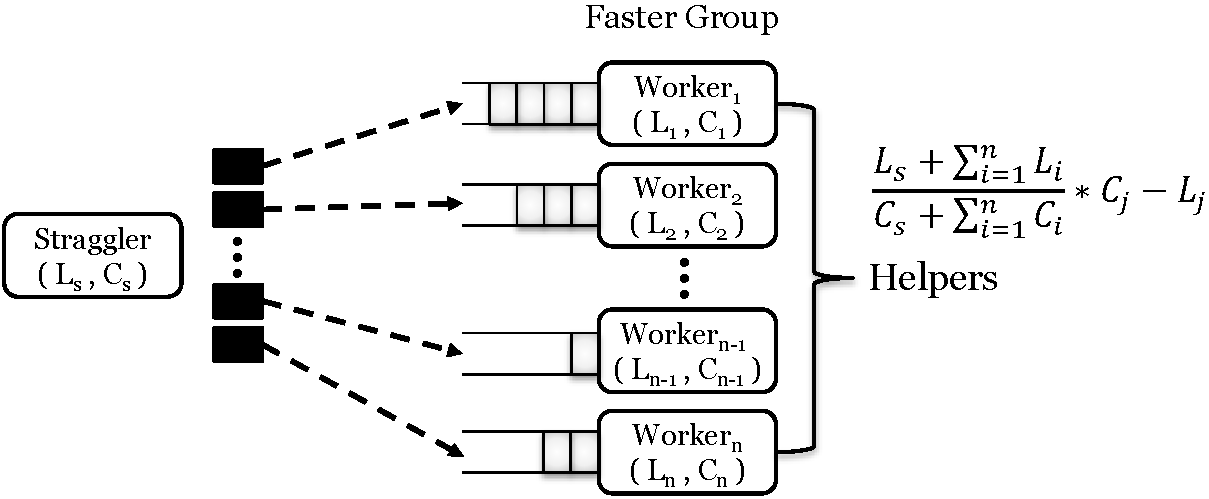
\includegraphics[width=0.48\textwidth]{FigureS1}
    \caption{All Strategy selects all nodes in faster group as helpers.}
    \label{Fig. 8:}
  \end{figure}

  \textbf{Two Choice Strategy.} Different from all strategy, two choice strategy chooses two nodes in faster group as helpers. Lever refers to the power of two choice\cite{Mitzenmacher1996} and intends to find out two nodes which have the large computational capability meanwhile have much less input data load as helpers. Fig. 9 shows the principle of two choice strategy. First, Lever sorts the nodes' list according to each node's \emph{$C_i$}/\emph{$L_i$} in the descending order. Then, Lever chooses the head two nodes as helpers and computes load share for each helper. Assume that the two selected helpers are $(C_1, L_1)$ and $(C_2, L_2)$, the straggler can be represented as (\emph{$C_s$},\emph{$L_s$}). The load share \emph{{$L_{sToj}$}} which is dispatched to jth helper can be denoted as:
  \begin{equation}
  L_{sToj} = \frac{L_s + L_1 + L_2}{C_s + C_1 + C_2}*C_j - L_j
  \end{equation}
  After reassignment, Lever updates each node's $C_i$ and $L_i$.
  \begin{figure}[htbp]
    \centering
    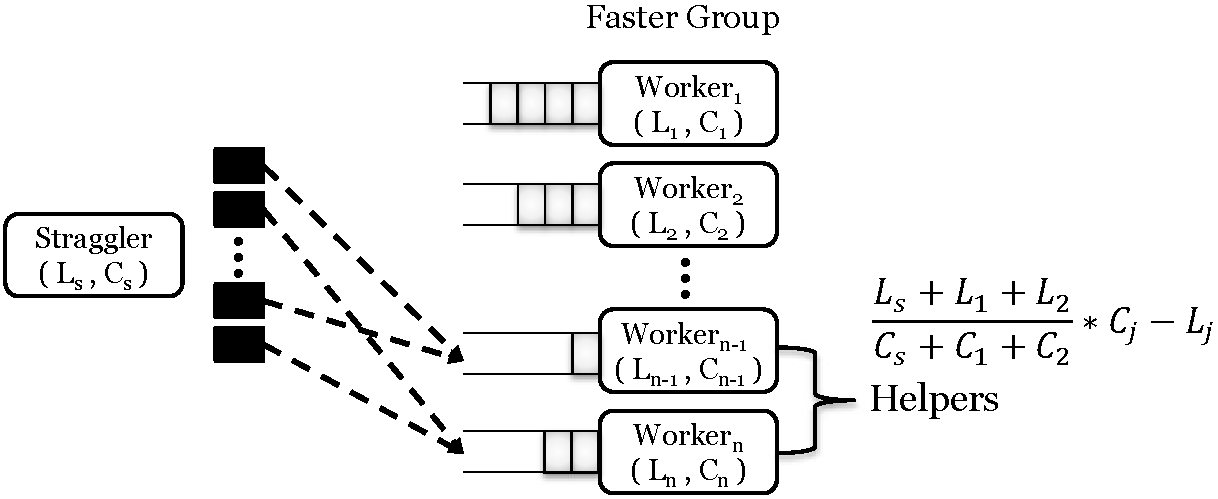
\includegraphics[width=0.48\textwidth]{FigureS2}
    \caption{Two Choice Strategy selects two nodes in faster group as helpers.}
    \label{Fig. 9:}
  \end{figure}

\subsubsection{Adaptively Choose One of Two}

  The above two strategies can be used in different situations. Lever can adaptively choose one of two strategies according to cluster's current state. Obviously, when there are few stragglers, all strategy is much better than two choice strategy because we can pre-schedule input data as evenly as possible. However, if there are large numbers of stragglers and fasters, two choice strategy will behavior better because of avoiding heavy blocks partition and migration. For example, if we have s stragglers and t fasters, this strategy will produce $s*t$ data pieces and also $s*t$ socket collections. Huge amount of $s*t$ value will incur network congestion and impact current jobs' execution.

  Lever combines the latency changes with the \#stragglers$\times$\#fasters to make adaptive choice. If \#stragglers$\times$\#fasters is larger than a observed value, Lever should select two choice strategy. Also another case is that when we detect that the latency of Lever is increasing after we adopt all strategy, then we will switch to two choice strategy. The complete pseudo code of pre-scheduling algorithm is presented in Algorithm 1.
  \begin{algorithm}[htbp]
  \small
  \caption{Pre-Scheduling Algorithm}
  \label{Alg:1}
  \begin{algorithmic}[1]
  \STATE \textbf{Procedure} \textbf{Identify Potential Stragglers}
  \STATE \quad Get the previous batches' job execution information
  \STATE \quad Sort the nodes descending by their finish time
  \STATE \quad Group the nodes into three groups(straggler, median, faster)
  \STATE \quad Compute the input load's gradient
  \STATE \quad Transform nodes' state according to transition rules
  \STATE \quad Output final stragglers and fasters
  \STATE \textbf{End Procedure}
  \STATE \textbf{Procedure} \textbf{Evaluate Computational Capability}
  \STATE \quad In ith batch, compute i+1th batch's capability
  \STATE \quad $C_{i+1} = C_i + C_i/t_i*(t_{ideal}-t_i)$
  \STATE \quad Assign corresponding load when receiving i+1th batch's data
  \STATE \quad In i+1th batch, compute the next batch's capability
  \STATE \quad $C_{i+2} = C_{i+1} + \frac{C_{i+1}}{t_{i+1}}*(t_{ideal}-t_{i+1})$
  \STATE \textbf{End Procedure}
  \STATE \textbf{Procedure} \textbf{Choose Suitable Helpers and Reassign Work}
  \IF{(\#stragglers$\times$\#fasters$<$$\rho$) or (last batch use AllStrategy \&\& latency decreases)}
  \STATE $/*$ continue to adopt allstrategy $*/$
  \STATE Choose all the nodes as helpers
  \STATE Compute the sum of helpers' capability and the sum of helpers' load
  \STATE $sumOfCapa=\sum_{i=1}^n C_i$ and $sumOfLoad=\sum_{i=1}^n L_i$
  \FOR{each straggler node}
  \FOR{each helper node}
  \STATE Compute the allocated load share
  \STATE $L_{stoi}=\frac{L_s + sumOfLoad}{C_s + sumOfCapa}\times C_i-L_i$
  \STATE Update each node's $(C_i,L_i)$
  \ENDFOR
  \ENDFOR
  \ELSE
  \STATE $/*$ adopt TwoChoiceStrategy $*/$
  \STATE Sort the nodes' list according to each node's $\frac{C_i}{L_i}$ in the descending order
  \STATE Choose the head two nodes as helpers
  \STATE Compute the sum of helpers' capability and the sum of helpers' load
  \STATE $sumOfCapa = C_1 + C_2$ and $sumOfLoad = L_1 + L_2$
  \FOR{each straggler node}
  \FOR{each helper node}
  \STATE Compute the allocated load share
  \STATE $L_{stoi}=\frac{L_s + sumOfLoad}{C_s + sumOfCapa}\times C_i-L_i$
  \STATE Update each node's $(C_i,L_i)$
  \ENDFOR
  \ENDFOR
  \ENDIF
  \STATE \textbf{End Procedure}
  \end{algorithmic}
  \end{algorithm}

\section{System Implementation}

  In this section, we describe the implementation of Lever. We have implemented Lever based on a popular open-source distributed, batched stream processing system called Spark Streaming \cite{spark-streaming}, which is an extension of cluster computing framework Apache Spark \cite{spark}. We choose Spark Streaming because it is a typical batched stream processing system based on Spark, a fast and general engine for large-scale data processing which powers a stack of libraries including SQL, machine learning, graph processing and stream processing. Spark Streaming has been widely adopted by academic community and industrial community, and also been deployed on production clusters of hundreds of thousands of corporations. In this section, we describe the details of our system implementation. The source code of our system can be found at \url{http://spark-packages.org/package/trueyao/spark-lever}.
  \begin{figure}[htbp]
    \centering
    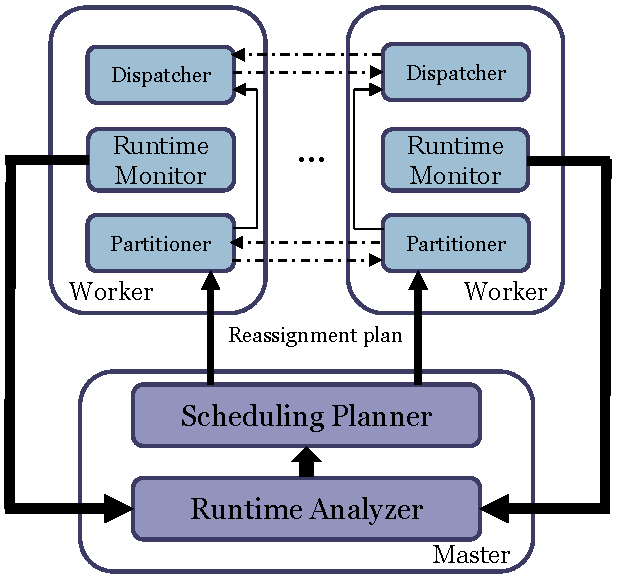
\includegraphics[width=0.35\textwidth]{Figure7}
    \caption{Implementation of Lever}
    \label{Fig. 10:}
  \end{figure}

  Figure 10 overviews the implementation of Lever. We add two components i.e. Runtime Analyzer and Scheduling Planner to master and three components i.e. Runtime Monitor, Partitioner and Dispatcher to worker, respectively. Runtime Monitor which locates in each worker periodically detects worker node information such as load and processing speed, then reports to Runtime Analyzer. By analyzing these information combined with jobs' detailed execution information, Runtime Analyzer identifies the stragglers and evaluate each node's computational capability. These results will be passed to Scheduling Planner for pre-scheduling decisions. Scheduling Planner should make a reassignment plan about how to partition and pre-schedule stragglers' work to other nodes. Partitioner is responsible for partition straggler's excess work according to specified proportion which is derived from Scheduling Planner. Dispatcher distributes every piece of partitioned work in current straggler to corresponding helpers.

  \textbf{Runtime Monitor.} \emph{Runtime Monitor} locates in each worker and periodically detects worker node information. We add some functions in \emph{executor}. When tasks are running in one executor, we can collect useful metrics such as task finish time and task's input data size through our function. We also add an accumulator in \emph{worker}. If there is one task completed, these metrics about this task is encapsulated into a message which will be sent to accumulator after this. Accumulator gathers these messages and reports to \emph{Runtime Analyzer} through an asynchronous RPC based on Akka.

  \textbf{Runtime Analyzer.} Once one batch has finished, \emph{Runtime Analyzer} begins to analyze the statistics information from \emph{Runtime Monitor}. We create a new component which maintains a table i.e. \emph{HashMap} in \emph{master}. This table is used for recording and updating workers' information. This component mainly consists of many massage receiving operations and two essential functions. One is for updating table, another is for identifying stragglers and evaluating capability.

  \textbf{Scheduling Planner.} This component receives messages from \emph{Runtime Analyzer}. It includes a main function which is responsible for running our capability-aware pre-scheduling algorithm and a output table which records pre-scheduling data assignment plan. And we also add some callback functions in \emph{JobScheduler} and \emph{TaskScheduler} in order to get scheduling information feedback and adjust task scheduling.

  \textbf{Partitioner.} We modify the \emph{BlockGenerator} and the \emph{ReceiverSupervisorImpl} to implement the Partitioner. We add a partition function \emph{splitBlockBuffer} to divide the receiving buffer into specified data share. And these fragments are delivered to \emph{BlockManager} as so called \emph{block} first(register the meta data such as block size and location to \emph{BlockManager}).

  \textbf{Dispatcher.} Function \emph{reallocateBlock} is the core of Dispatcher. This component carry out two things. One is getting the host name which data piece will be assigned to from the assignment plan. And another is invoking the \emph{blockTransferService} to transfer block. We modify the system call \emph{uploadBlockSync} in Lever to implement the remote block assignment.

\section{Experimental Evaluation}

  In this section, we evaluate Lever's performance using various workloads. First, we describe the experimental environment, and then present the experimental results.

\subsection{Experimental Setup and Workloads}

  \textbf{Experimental Setup.} Our evaluations are conducted on a heterogeneous cluster consisting of two types of machines with different configurations. The first kind of machines is comprised of two dual-core Intel Xeon E5-2670 2.6 GHz CPUs, 16GB memory, and 210GB disks. The second kind of machines consists of two dual-core 1.2 GHz Intel CPU, 4GB memory, and 210GB disks. All computers are interconnected with 1Gbps Ethernet cards. We use spark-1.3.0 as the distributed computing platform and Redhat Enterprise Linux 6.2 with the kernel version 2.6.32 as the OS.

  \textbf{Workloads.} Table \uppercase\expandafter{\romannumeral2} describes the benchmarks used in our experiments. Similar to previous work \cite{Zaharia2013}, we choose three typical applications i.e. Grep, WordCount, and TopK. In addition, we also use the HiBench \cite{HiBench} benchmark including Identity, Sample and Projection. We rewrite the HiBench \cite{HiBench} benchmark based on receiver model. We use the real datasets of internet traffic archive available in \cite{datasets} as stream data source.
  \begin{table*}[htbp]
    \footnotesize
    \centering
    \caption{Benchmarks}
    \begin{threeparttable}
    \centering
      \begin{tabular}{|p{1.4cm}|p{7.2cm}|p{1.5cm}|p{2.8cm}|p{1.7cm}|}
        \hline
        \centering
        \textbf{Benchmark} & \textbf{Description} & \textbf{Complexity} & \textbf{Resource Preference} & \textbf{Source} \\
        \hline
        Identity & Simply reads input and takes no operations on it & Single Step & None & HiBench \cite{HiBench} \\
        \hline
        Sample & Samples the input stream according to specified probability & Single Step & None & HiBench \cite{HiBench} \\
        \hline
        Projection & Extracts a certain field of the input & Single Step & Network Intensive & HiBench \cite{HiBench} \\
        \hline
        Grep & Checks if the input contains certain strings & Single Step & Network Intensive & DStream \cite{Zaharia2013} \\
        \hline
        WordCount & counts the number of each word in input text & Multi Step & CPU Intensive & DStream \cite{Zaharia2013} \\
        \hline
        Topk & Finds the k most frequent words over the specified window & Multi Step & CPU Intensive & DStream \cite{Zaharia2013} \\
        \hline
      \end{tabular}
    \end{threeparttable}
    \label{Table2}
  \end{table*}

  \textbf{Other configurations.} In all our experiments, we use default data locality wait time(3s), therefore Delay Scheduling \cite{Zaharia2010B} doesn't not interfere with our experimental results. For speculation, we set the speculation interval, speculation quantile(default 0.75) and speculation multiplier(default 1.5) as 100ms, 0.5, 1 respectively. These settings can let speculative execution perform much best in our environment. We implement Skewtune, Dolly and Wrangler's prototypes. We adopt local scan for skewtune. We also set wait duration of delay assignment $\omega$ as 200ms in Dolly. For Wrangler, we set confidence measure $\rho$ as 0.7 and set interval(decides how frequently a snapshot of node's resource usage counters is collected) $\Delta$ as one batch.

  Unless specified otherwise, we use 2s' batch interval and 100-bytes input records. Stragglers are on average 8 times slower than the median task in each job. All input data blocks only have one replica. We don't fetch the final results until the results are stable after each benchmark runs about 10 minutes. Each experiment is repeated five times and we present the median numbers. The baseline is original spark streaming with speculation closed.

\subsection{Job Completion Time}

  We first test the improvement in completion time using Lever. Figure 11 reports the normalized job completion time when compared with other strategies. Lever can significantly improve performance when running Projection, Grep, WordCount and Topk. But Lever improves a little for Identity and Sample relatively. It depends on the type of workloads. Identity and Sample are of simple execution logic. Straggler has little impact on these workloads.

  Compared to baseline, Lever improves the average job completion time by 32.31\%, 30.72\%, 37.54\% and 42.19\% for Projection, Grep, WordCount and Topk, respectively. Speculation and Skewtune works much worse in our experiments because they need to speed a long time on detecting stragglers and data skew. Lever pre-schedules job input data before task scheduling and avoid the detecting and migrating overhead. As a result, Lever outperforms other strategies for the performance of Projection(by up to 29.47\%, 32.06\%, 22.99\% and 25.56\% compared to Speculation, Skewtune, Dolly and Wrangler), Grep(by up to 28.87\%, 29.11\%, 18.82\% and 25.81\% compared to Speculation, Skewtune, Dolly and Wrangler), WordCount(by up to 33.33\%, 37.37\%, 31.11\% and 28.74\% compared to Speculation, Skewtune, Dolly and Wrangler) and Topk(by up to 34.48\%, 41.24\%, 34.48\% and 31.33\% compared to Speculation, Skewtune, Dolly and Wrangler).
  \begin{figure}[htbp]
    \centering
    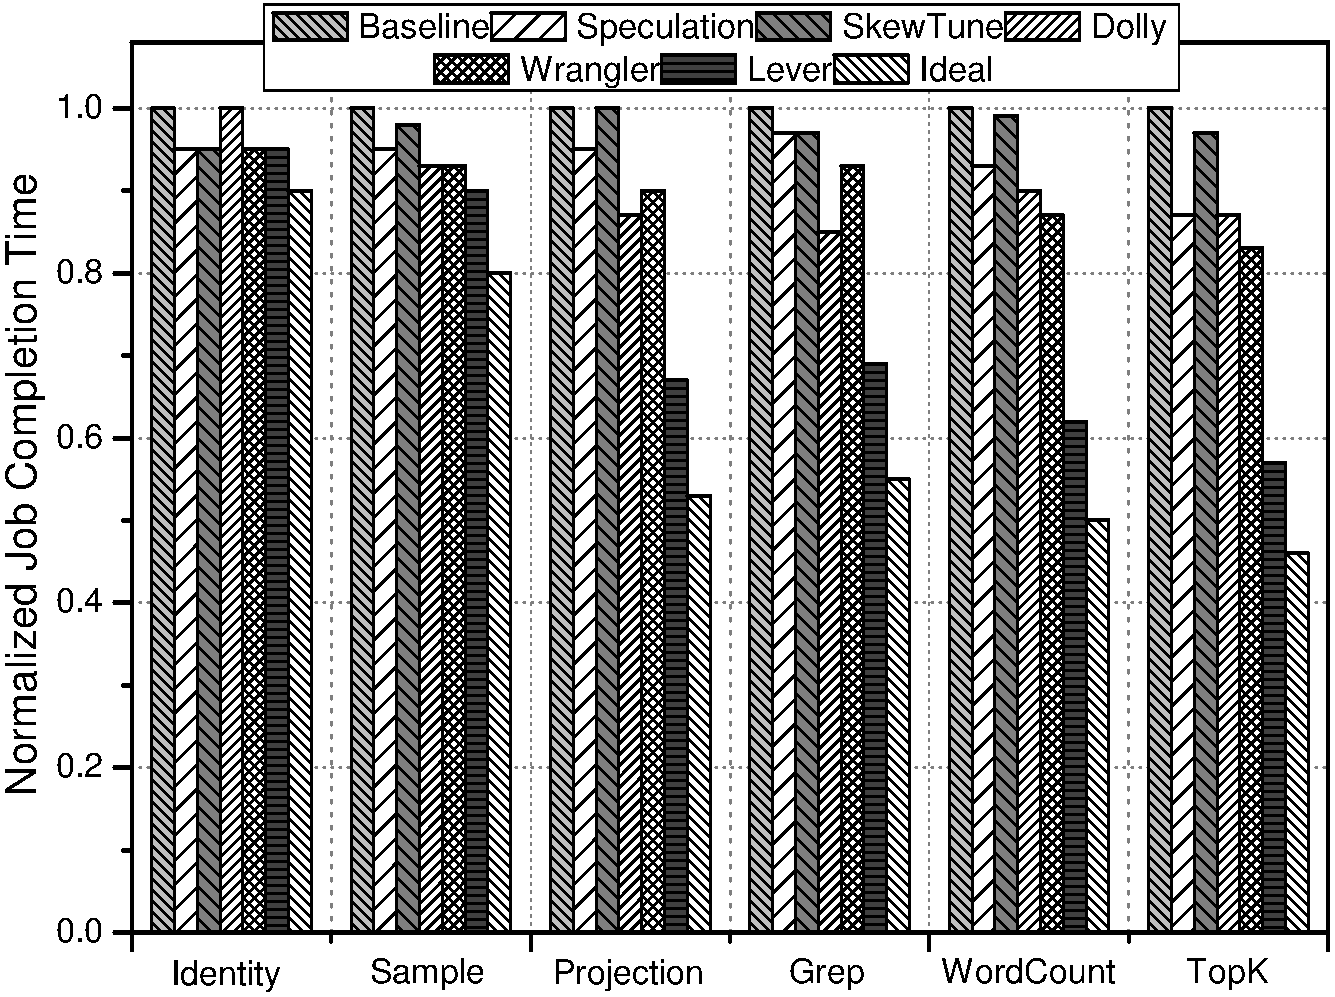
\includegraphics[width=0.35\textwidth]{FigureJCT}
    \caption{Normalized job completion time when running benchmarks under different techniques}
    \label{Fig. 11:}
  \end{figure}

  Figure 12 shows a detailed analysis of task completion time in three types of nodes. We average task's completion time of faster group, median group and straggler group. Task's completion time in each node decides the makespan of this job. As we can see, straggler is quite remarkable under traditional methods. It means that these techniques cannot eliminate stragglers very well. As a result, the straggler nodes are load-heavy all the batch and the fasters are idle for a long time. It is due to their fumbling reaction to stragglers. In the ideal case, all the nodes should complete their tasks at almost the same time. Lever behaviors much better because it balances data skew when receiving data. So when tasks are running, all nodes can progress at almost the same rate.
  \begin{figure}[htbp]
    \centering
    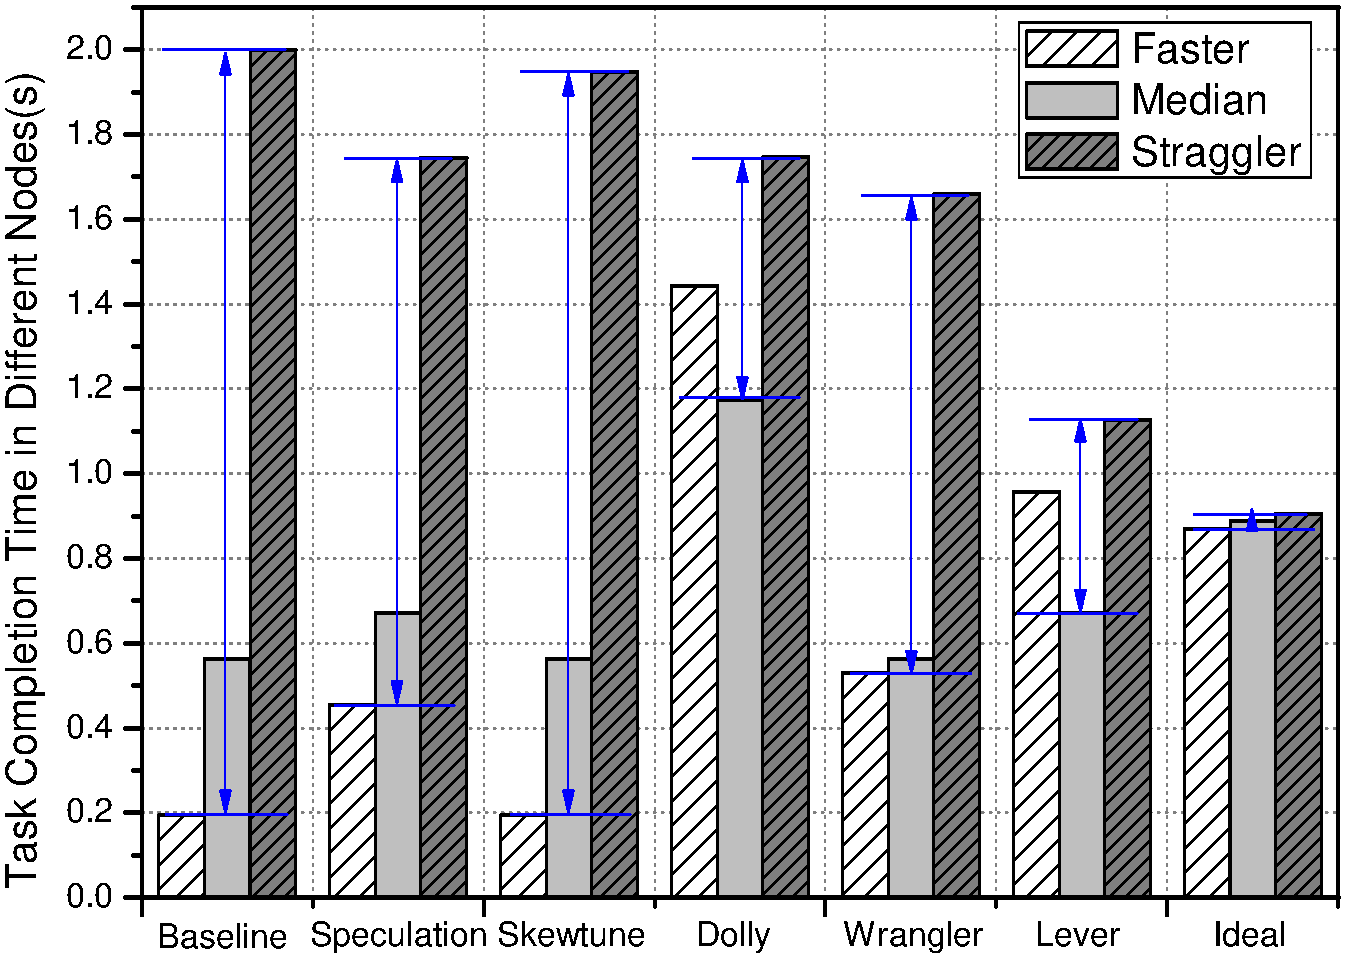
\includegraphics[width=0.32\textwidth]{FigureMakeSpan}
    \caption{Task completion time in three types of nodes when running WordCount}
    \label{Fig. 12:}
  \end{figure}

  Table \uppercase\expandafter{\romannumeral3} lists the node's idle time when a batch is completed. Baseline and Skewtune waste more than 3s for faster and median nodes totally in a 2s' batch interval. Speculation and Wrangler are idle for about 2s. Much of this time is spent on detection and migration. This is the root cause of why they perform much worse than others. Although Dolly wastes less time, it clones tasks, which means that it need to complete 2x amount of work. Lever also has idle time as long as 0.625s. This is because Lever only takes the straggler and faster into account regardless of median group's node. For median, it is difficult to estimate whether it will be faster or slower than stragglers after we redistribute load.
  \begin{table*}[htbp]
    \small
    \centering
    \caption{Node's idle time for faster and median}
    \begin{threeparttable}
    \centering
      \begin{tabular}{|p{1.4cm}|p{1.2cm}|p{1.5cm}|p{1.2cm}|p{0.9cm}|p{1.2cm}|p{0.9cm}|p{0.9cm}|}
        \hline
        Techniques & Baseline & Speculation & Skewtune & Dolly & Wrangler & Lever & Ideal \\
        \hline
        Idle time & 3.243s & 2.363s & 3.137s & 0.875s & 2.224s & 0.625s & 0.055s \\
        \hline
      \end{tabular}
    \end{threeparttable}
    \label{Table3}
  \end{table*}

  In summary, Lever saves a lot of idle time through pre-scheduling data assignment, thus avoiding detection, migration and cloning. So Lever can mitigate stragglers and improve the performance significantly.

\subsection{Adaptability for burst load}

  In this testing scenario, we give one node burst load to evaluate the robustness and the convergence time of Lever. The burst load results in that task completion time exceeds greatly than batch interval. We also test other techniques' effectiveness under this situation.

  From the test result in Figure 13, we observe that both Lever and Wrangler can achieve much better performance. Baseline, Speculation, Skewtune and Dolly can't process subsequent jobs timely because their cloning and hysteresis reaction aren't not enough, leading a large number of subsequent jobs are queueing in scheduler's waiting queue. The scheduling delay will increases monotonously.

  Although Wrangler can go on processing subsequent jobs, Wrangler is not stable enough with delay jitter. This is because Wrangler only cares about stragglers in one batch. The nodes of light load(actually are potential stragglers) in current batch will be scheduled many tasks in the next batch, leading to nodes being overloaded.

  Lever avoids this problem by analyzing recurring jobs' load fluctuation in previous batches. As shown in Figure 13, Lever can converge to an ideal latency in six batches. The estimation for capability by using ILC also returns to normal in six batches after experiencing a short period of fluctuations.

  In summary, Lever can adapt to burst load effectively and converge to a steady state quickly.
  \begin{figure}[htbp]
    \centering
    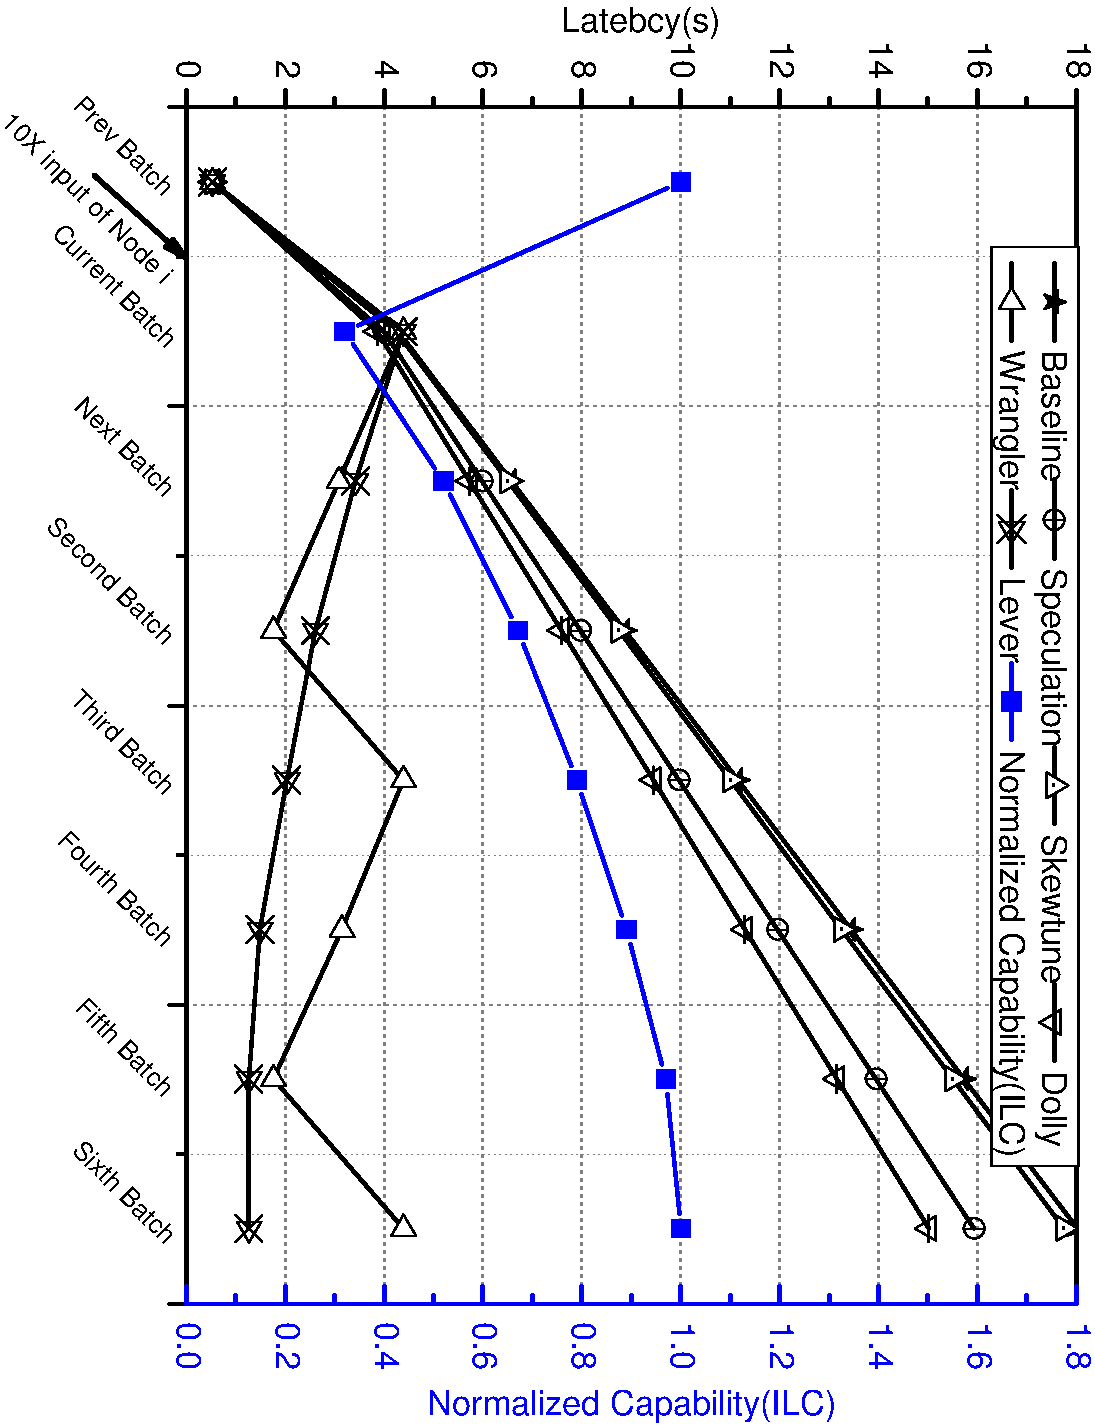
\includegraphics[width=0.30\textwidth, angle=90]{FigureAdapBurst}
    \caption{Latency and Normalized Capability when running WordCount under burst load}
    \label{Fig. 13:}
  \end{figure}

\subsection{Data Locality and Queued Tasks}

  \begin{figure}[htbp]
    \centering
    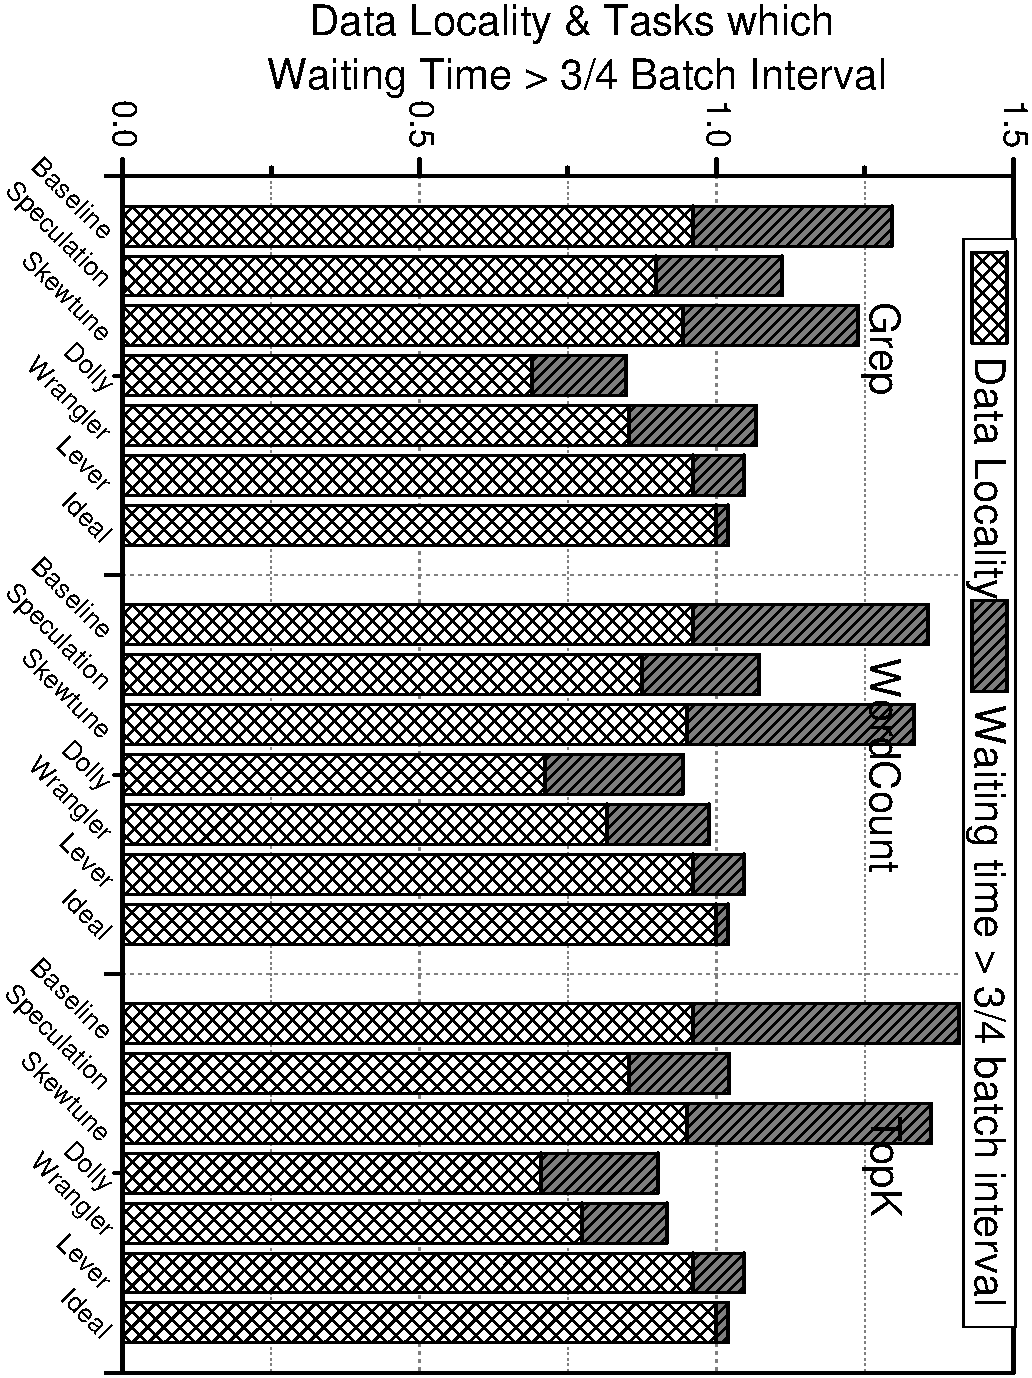
\includegraphics[width=0.28\textwidth, angle=90]{FigureDLWT}
    \caption{Data Locality and Tasks which waiting time is greater than 3/4 batch interval when running Grep, WordCount and Topk}
    \label{Fig. 14:}
  \end{figure}

  In this test, we conduct a statistical analysis about data locality and queued tasks which waiting time is greater than three quarters of batch interval. We observe that in our experiments if a task waits for three quarters of batch interval, it means that this node is overloaded and the batch processing time will exceed the batch interval.

  As shown in Figure 14, for Baseline, although most of the tasks can execute in the local node, there are 33.5\%, 39.7\%, 44.9\% tasks waiting for more than three quarters of batch interval for Grep, WordCount and Topk, respectively. These tasks are from straggler nodes. In order to illustrate the difference, we take WordCount for example. Dolly and Wrangler only have up to 23.1\% and 17.3\% tasks waiting for more than three quarters of batch interval. However, they only have 71.2\% and 81.5\% node local tasks. They need to migrate tasks to remote nodes at runtime. This migration causes extra overhead and neutralizes benefits from reduction in the number of waiting tasks. Speculation only detects and migrates a small number of tasks. Skewtune performs much worse because it spends so long time on detection that it can't react to straggler and data skew quickly.

  In the ideal case, all nodes execute local tasks and there aren't tasks queued for three quarters of batch interval. Lever can achieve 96\% data locality and 8.7\% waiting tasks. The reason why Lever can not reach the ideal state is that Lever relies on the estimation of node's capability and Lever ignores the median nodes. This impedes Lever's perfect load balancing.

  In summary, compared to other strategies, Lever can achieve better data locality and reduce the number of tasks which waiting for a long time.

\subsection{All Strategy or Two Choice Strategy}

  In this test scenario, we compare two helper-choosing strategies when faced with different straggler situations. We varies the number of stragglers and the number of fasters to evaluate the advantages and disadvantages of two methods.

  The experimental results presented in Figure 15 show that when there are few stragglers in current cluster, allStrategy is much better than twoChoiceStrategy. However, if there are more and more nodes will be stragglers, twoChoiceStrategy behave much better. We give an example to elaborate the reason. Assume that we have n stragglers and m fasters, allStrategy produces n$\times$m partitions to migrated and rebalanced, but twoChoiceStrategy only produces n$\times$2 fragmentations. Although allStrategy makes load well-distributed, which accompany with it is the increasing overhead in partition and network transformation.

  In our experiments, when there are 8 stragglers and 10 fasters, twoChoiceStrategy begins to perform better than allStrategy. It means that when the observed value $\rho$ is larger than 80, then Lever should choose twoChoiceStrategy. As shown in Figure 15, Lever can select helper-choosing strategies adaptively according to straggler situations and latency fluctuation.
  \begin{figure}[htbp]
    \centering
    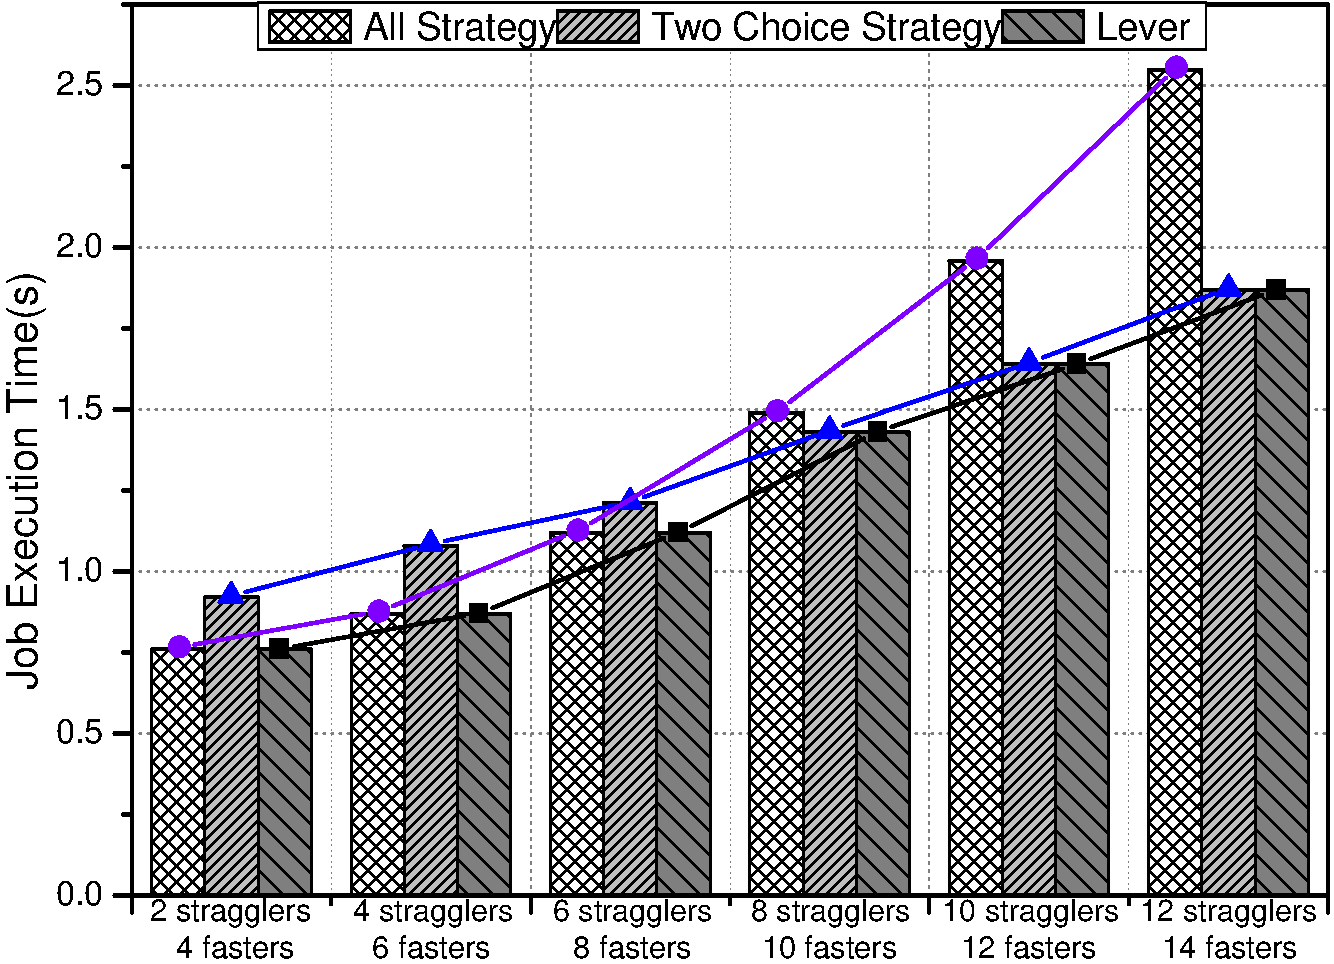
\includegraphics[width=0.35\textwidth]{FigureAllorTwo}
    \caption{Results under different straggler situations using two strategies}
    \label{Fig. 15:}
  \end{figure}

  In summary, allStrategy is suitable for few stragglers and few fasters and twoChoiceStrategy is more suitable for many stragglers or many fasters. Lever can choose one of the two adaptively to ensure the performance.

\section{Related Work}

  Our work is related to the research in batched stream processing and straggler mitigation on heterogeneous clusters. We briefly discuss the most related work.

  \textbf{Batched Stream Processing and Incremental Data Processing Systems.} Batched stream processing systems collect received data into batches and periodically process them using MapReduce-style batch computations. The typical systems include Comet \cite{He2010} which is structured on DryadLINQ, HOP \cite{Condie2010} which leverages the power of batch framework MapReduce, and Spark Streaming \cite{Zaharia2013} which is built on top of Spark. These systems take full advantage of characteristics in batch processing engine such as high throughput and fault-tolerance. Some other systems \cite{Li2011} and \cite{Lam2012} intent to modify batch framework to adapt to the requirements of stream processing. Other stream processing systems such as Borealis \cite{Abadi2005}, TimeStream \cite{Qian2013}, Naiad \cite{Murray2013}, Storm \cite{Toshniwal2014} and Heron \cite{Kulkarni2015} are based on the \emph{continuous operator model}. In this model, the streaming computation is expressed as a graph of long-lived operators that exchange messages with each other to process the streaming data.Incremental bulk processing systems such CBP \cite{Logothetis2010}, Percolator \cite{Peng2010} and Incoop \cite{Bhatotia2011a} allows updated view of processed data set to be maintained by incrementally and efficiently recomputing the updates to the input data. In such systems, the recomputation is triggered whenever an update to the input dataset is detected.

  \textbf{Straggler and Data Skew on Heterogeneous Clusters.} Load imbalance on heterogeneous clusters are common phenomenon in cluster computing environments because of heterogeneity, straggler, data skew and so on. Many techniques have been presented to solve these problems. The typical scheduling methods are Delay Scheduling \cite{Zaharia2010B}, LATE \cite{Zaharia2008}, and Tarazu \cite{Ahmad2012}. Delay Scheduling tries to maintain data locality by later decision. LATE speculates slow tasks using a notion of progress scores. Tarazu designs communication-aware load balancing of map computation, communication-aware scheduling of map computation, and predictive load balancing of reduce computation to respectively prevent shuffle-critical tasks stealing, interleave remote tasks with local ones, and skew the intermediate key distribution among the reduce tasks. They are reactive ways for batch processing. The typical straggler mitigation approaches are Speculative Execution \cite{Dean2004}, Mantri \cite{Ananthanarayanan2010}, Dolly \cite{Ananthanarayanan2013}, GRASS \cite{Ananthanarayanan2014} and Wrangler \cite{Yadwadkar2014}. Speculative Execution marks slow tasks as stragglers and launch a redundant copy of a task-in-progress on a different node. Using real-time progress reports, Mantri monitors, detects and acts on outliers by restarting outliers, network-aware placement of tasks and protecting outputs of valuable tasks. Dolly is a replication-based method, it proposes full cloning of small jobs by delay assignment. Dolly don't need to wait to observe before acting with a proactive approach of cloning jobs. But it incurs extra resources. GRASS is designed for approximation jobs, it delicately balances immediacy of improving the approximation goal with the long term implications of using extra resources for speculation. Wrangler automatically learns to predict stragglers using a statistical learning technique based on cluster resource utilization counters. It is a straggler-avoid method.The typical skew mitigation techniques are Scarlett \cite{Ananthanarayanan2011}, SkewTune \cite{Kwon2012}. Scarlett replicates block based on their popularity by accurately predicting file popularity and working within hard bounds on additional storage.SkewTune solves the problem of load balancing in MapReduce-like systems by identifying the task with the greatest expected remaining processing time and redistributing the unprocessed data from the stragglers to other workers.

\section{Conclusion}

  This paper presents Lever, a pre-scheduling straggler mitigation framework that exploits the predictability of recurring batched stream jobs to optimize the assignment of data. Lever identifies potential stragglers by analyzing execution information of historical jobs and introduces Iterative Learning Control(ILC) model to evaluate nodes' capability. Furthermore, Lever carefully chooses helpers and optimizes the assignment of the job input data according to each node's capability proportion. Lever has been implemented on the top of Spark Streaming. Lever is also open source and is now included in Spark Packages at \url{http://spark-packages.org/package/trueyao/spark-lever}. We conduct various experiments to validate the effectiveness of Lever. The experimental results demonstrate that Lever reduces job completion time by 30.72\% to 42.19\% and outperforms traditional techniques significantly.

  In future work, we plan to enhance the accuracy for estimation of node's computational capability. A possible approach is to introduce a new machine learning method to evaluate each node by collecting the node-level features of hardware configuration and resource utilization such as CPU, memory, disk and network. By using a statistical model to analyze these information, we can get a relatively more accurate result to direct capability-aware pre-scheduling. Another direction in the future is that we will consider the influence of shuffle-heavy tasks and how to balance load at shuffle stage. It will extend the usage of Lever.

%\section*{Acknowledgment}

%  This work was supported by National Science Foundation of China under grant No.61472151 and No.61232008, National 863 Hi-Tech Research and Development Program under grant No.2014AA01A302 and No.2015AA01A203, the Fundamental Research Funds for the Central Universities under grant No.2015TS067.

\bibliographystyle{IEEEtran}
\bibliography{MyCollection}

\end{document}


